\documentclass{article}
\usepackage{amsfonts} % For \mathbb
\usepackage{amsmath} % For align*
\usepackage{enumitem} % For customisable list labels
\usepackage{graphicx} % For images
\usepackage{siunitx} % For units
\graphicspath{{./images/}}

\title{University Physics with Modern Physics - Modern Physics by Young and Freedman Notes}
\author{Chris Doble}
\date{June 2023}

\begin{document}

\maketitle

\tableofcontents

\setcounter{section}{16}
\section{Temperature and Heat}

\subsection{Temperature and Thermal Equilibrium}

\begin{itemize}
  \item The \textbf{zeroth law of thermodynamics} states: If $C$ is initially in thermal equilibrium with both $A$ and $B$, then $A$ and $B$ are also in thermal equilibrium with each other.

  \item Two systems are in thermal equilibrium iff they have the same temperature.
\end{itemize}

\subsection{Thermometers and Temperature Scales}

\begin{itemize}
  \item Water freezes at $\ang{0} \unit{C}$ or $\ang{32} \unit{F}$ and boils at $\ang{100} \unit{C}$ or $\ang{212} \unit{F}$.

  \item A temperature measurement is denoted $x \unit{\degree C}$ (``$x$ degrees Celsius'') whereas a temperature interval is denoted $x \unit{C \degree}$ (``$x$ Celsius degrees'').
\end{itemize}

\subsection{Gas Thermometers and the Kelvin Scale}

\begin{itemize}
  \item Under the \textbf{Kelvin} temperature scale temperature differences are equal to those of the degrees Celsius scale, but the zero is equal to $\ang{-273.15} \unit{C}$. This is known as \textbf{absolute zero} where molecules have their lowest possible kinetic and potential energies.

  \item The ratio of two temperatures in the Kelvin scale equals the ratio of the corresponding pressures in a constant-volume gas thermometer \[\frac{T_2}{T_1} = \frac{p_2}{p_1}.\]
\end{itemize}

\subsection{Thermal Expansion}

\begin{itemize}
  \item Materials expand when their temperatures increase.

  \item Expansion in a single dimension is described by the equation \[\Delta L = \alpha L_0 \Delta T\] where $\Delta L$ is the change in length, $\alpha$ is the \textbf{coefficient of linear expansion}, $L_0$ is the original length, and $\Delta T$ is the change in temperature.

  \item Expansion in three dimensions (volume expansion) is described by the equation \[\Delta V = \beta V_0 \Delta T\] where $\Delta V$ is the change in volume, $\beta$ is the \textbf{coefficient of volume expansion} (equal to $3 \alpha$), $V_0$ is the original volume, and $\Delta T$ is the change in temperature.

  \item If the ends of a material are fixed in place, changes in temperature can induce \textbf{thermal stresses} that can damage the material. The magnitude of these stresses is given by \[\frac{F}{A} = -Y \alpha \Delta T.\]
\end{itemize}

\subsection{Quantity of Heat}

\begin{itemize}
  \item Energy transferred as a result of a temperature difference is called \textbf{heat}.

  \item The \textbf{specific heat} of a material is the amount of energy required to raise the temperature of one unit of mass of the material by one unit of temperature, e.g. $\qty{1}{kg}$ by $\qty{1}{K}$. It has units like $\unit{J/(kg.K)}$.

  \item The specific heat of water is \[\qty{4190}{J/(kg.K)} \text{ or } \qty{1}{cal / (g.C\degree)}.\]

  \item The energy required to change the temperature of a material is given by \[Q = m c \Delta T\] where $m$ is the mass of the material, $c$ is its specific heat, and $\Delta T$ is the change in temperature.

  \item The \textbf{molar mass} of a substance is the mass of one mole.

  \item The total mass of a material $m$ is equal to the mass per mole $M$ times the number of moles $n$ \[m = n M.\]

  \item The energy required to change the temperature of a certain number of moles of a substance is \[Q = n C \Delta T\] where $C = M c$ is the \textbf{molar heat capacity}.
\end{itemize}

\subsection{Calorimetry and Phase Changes}

\begin{itemize}
  \item A \textbf{phase} is a specific state of matter, e.g. solid, liquid, or gas.

  \item A \textbf{phase change} or \textbf{phase transition} is a transition from one phase to another.

  \item For a given pressure, phase change takes places at a definite temperature.

  \item While a substance is undergoing a phase change, any added or removed energy will affect the progress of the phase change but won't change the temperature.
\end{itemize}

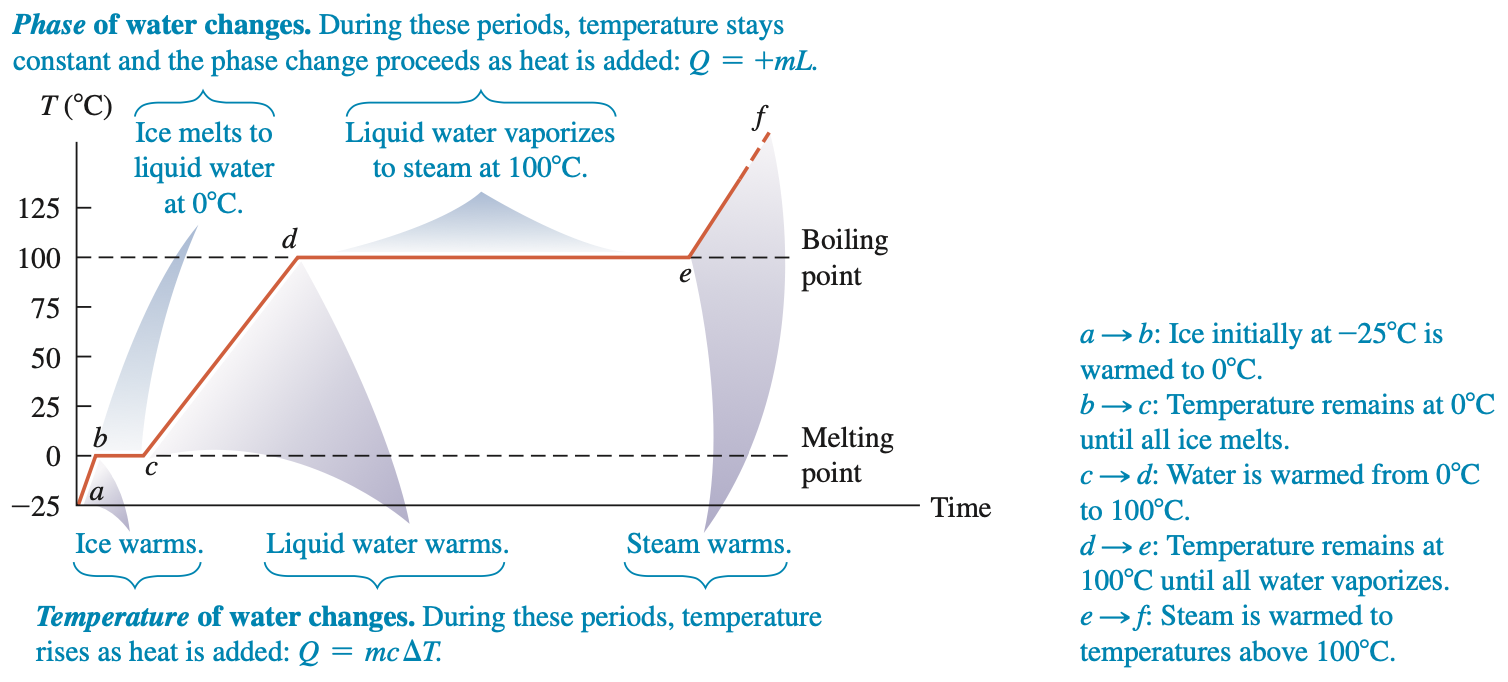
\includegraphics[scale=0.43]{phase-vs-temperature}

\begin{itemize}
  \item The heat transfer required for a material to undergo a phase change is given by \[Q = \pm m L\] where the $\pm$ indicates that heat may need to be added or removed depending on the direction of the phase change (e.g. energy must be added to melt ice), $m$ is the mass of the material, and $L$ is the latent heat associated with the phase change.

  \item When a material is freezing or melting, $L = L_f$ the \textbf{latent heat of fusion}.

  \item When a material is condensing or vaporising, $L = L_v$ the \textbf{latent heat of vaporisation}.

  \item When a material sublimates (changes directly from a solid to a gas, skipping liquid) or deposits/desublimates (changes directly from a gas to a solid, skipping liquid), $L = L_s$ the \textbf{latent heat of sublimation}.

  \item When a material burns, $L = L_c$ the \textbf{latent heat of combustion}.

  \item For any given material at any given pressure, the freezing temperature is the same as the melting temperature. This is called \textbf{phase equilibrium}. Similarly the condensing temperature is the same as the vaporisation temperature.
\end{itemize}

\subsection{Mechanisms of Heat Transfer}

\begin{itemize}
  \item \textbf{Conduction} is a mechanism of heat transfer where the molecules in an area of high temperature have greater kinetic energy, they bump neighboring molecules which increases their kinetic energy, and so on spreading the heat through the material.

  \item The direction of heat flow is always from higher to lower temperature.

  \item When a quantity of heat $dQ$ is transferred through a material in time $dt$ we say the rate of heat flow or the \textbf{heat current} is \[H = \frac{dQ}{dt}.\]

  \item If a rod has cross sectional area $A$, length $L$, one end is held at temperature $T_H$, and the other is held at $T_C$ where $T_H > T_C$, the heat current is \[H = \frac{d Q}{d T} = k A \frac{T_H - T_C}{L}\] where $k$ is the \textbf{thermal conductivity} of the material and $(T_H - T_C) / L$ is the temperature difference per unit length or the magnitude of the \textbf{temperature gradient}.

  \item \textbf{Convection} is the transfer of heat by mass motion of fluid from one region of space to another, e.g. ducted cooling/heating. If the fluid is circulated by a blower or a pump the process is called \textbf{forced convection}; if the flow is caused by differences in density due to thermal expansion, such as hot air rising, the process is called \textbf{free convection}.

  \item \textbf{Radiation} is the transfer of heat by electromagnetic waves such as visible light, infrared, and ultraviolet radiation.

  \item The wavelength of the radiation depends on temperature. At $\qty{20}{\degree C}$ the radiation is infrared. At $\qty{800}{\degree C}$ the radiation is red. At $\qty{3000}{\degree C}$ the radiation is white.

  \item The \textbf{Stefan-Boltzmann law} gives the rate of energy radiation from a surface \[H = A e \sigma T^4\] where $A$ is its surface area, $e$ is a dimensionless constant between 0 and 1 called the \textbf{emissivity} of the surface (1 would be a perfect radiator), $\sigma$ is the \textbf{Stefan-Boltzmann constant} \[\sigma = \qty{5.67037442e-8}{W/(m^2.K^4)},\] and $T$ is the temperature in Kelvin.

  \item An object's surroundings also emit radiation which is absorbed by the object. The net heat current from the object is this \[H = A e \sigma (T^4 - T_s^4)\] where $T_s$ is the temperatue of the surroundings. At thermal equilibrium there is no heat flow.

  \item An object that is a good absorber must also be a good emitter. An ideal radiator with $e = 1$ is also an ideal absorber, absorbing all the raditation that hits it. Such a surface is called an \textbf{ideal black body} or a \textbf{blackbody}.
\end{itemize}

\section{Thermal Properties of Matter}

\subsection{Equations of State}

\begin{itemize}
  \item Quantities such as pressure, volume, temperature, and amount of substance are called \textbf{state variables}.

  \item An equation that relates state variables is called an \textbf{equation of state}.

  \item Molar mass (i.e. the mass of one mole of a substance) is sometimes called \textbf{molecular weight}.

\item The \textbf{ideal gas equation} relates the absolute pressure $p$, volume $V$, number of moles $n$, and absolute temperature (in Kelvin) $T$ \[p V = n R T\] or \[p V = \frac{m_\text{total}}{M} RT\] or \[p V = N k T\] where $R$ is the gas constant \[R = \qty{8.314}{J/(mol.K)}.\]

  \item If the amount of a gas is contant, i.e. $n R$ is constant, then \[\frac{p_1 V_1}{T_1} = \frac{p_2 V_2}{T_2} = \text{constant}.\]

  \item \textbf{Standard temperature and pressure} (STP) is defined as $\qty{0}{\degree C}$ and $\qty{1}{atm}$.

  \item The \textbf{van der Waals} equation extends the ideal gas law to account for the effects of interactions between gas molecules and their finite size \[\left( p + \frac{a n^2}{V^2} \right) (V - n b) = n r T\] where $a$ and $b$ are constants that vary between gases, $a$ depends on the strength of attractive forces between the molecules, and $b$ depends on the volume of the molecules.

  \item A $p V$-diagram is a two-dimensional diagram plotting pressure as a function of volume. Each line, called an \textbf{isotherm}, describes the relationship between pressure and volume at a particular temperature.

  \item In the $p V$-diagrams of non-ideal gases, isotherms can have flat areas. These represent periods where the gas is condensing into a liquid.

  \item The area under a $p V$-curve represents the work done by the system during a volume change.
\end{itemize}

\subsection{Molecular Properties of Matter}

\begin{itemize}
  \item The force between molecules in a gas varies with $r$.

  \item An ideal gas is one whose molecules exert no attractive forces on each other and thus have no potential energy.

  \item The number of molecules in a mole is given by \textbf{Avagadro's number} \[N_A = \num{6.02214076e23} \,\text{molecules}/\text{mol}.\]
\end{itemize}

\subsection{Kinetic-Molecular Model of an Ideal Gas}

\begin{itemize}
  \item The average translational kinetic energy of an ideal gas is \[K_\text{tr} = \frac{3}{2} n R T.\]

  \item The \textbf{Boltzmann constant} is \[k = \frac{R}{N_A} = \num{1.381e-23} \,\text{J}/(\text{molecule K}).\]

  \item The average translational kinetic energy of a gas molecule is \[\frac{1}{2} m (v^2)_\text{av} = \frac{3}{2} kT\] and thus the \textbf{root-mean-square speed} of a gas molecule is \[v_\text{rms} = \sqrt{(v^2)_\text{av}} = \sqrt{\frac{3 k T}{m}} = \sqrt{\frac{3 R T}{M}}\] where $m$ is the mass of a molecule and $M$ is the molar mass.

  \item The average distance travelled by a particle between collisions is called the \textbf{mean free path} \[\lambda = \frac{V}{4 \pi \sqrt{2} r^2 N} = \frac{k T}{4 \pi \sqrt{2} r^2 p}\] where $V$ is the volume of the gas, $r$ is the radius of a gas molecule, $N$ is the number of molecules in the gas, $T$ is its temperature, and $p$ is its volume.
\end{itemize}

\subsection{Heat Capacities}

\begin{itemize}
  \item The \textbf{molar heat capacity at constant volume} of a particular gas is determined by its \textbf{degrees of freedom}, i.e. the number of ways in which it can store kinetic energy.

        \begin{itemize}
          \item Monatomic gases have three degrees of freedom: one for each translational axis.

          \item Diatomic gases have five degrees of freedom: one for each translational axis and two for rotational axes (the third is excluded because it's not affected by collisions).

          \item Polyatomic gases have more than five degrees.
        \end{itemize}

\item The \textbf{principle of equipartition of energy} states that each degree of freedom contributes $\frac{1}{2} k T$ to the average kinetic energy of the gas, i.e. for monatomic gases the average kinetic energy per molecule is $\frac{3}{2} k T$, for diatomic $\frac{5}{2} k T$, etc.

\item The molar heat capacity at constant volume of a gas is equal to \[C_V = \frac{d}{2} R\] where $d$ is the number of degrees of freedom.

  \item Vibrational energy can also contribute to the molar heat capacity at constant volume, but for most diatomic molecules this isn't the case.

  \item Molar heat capacity at constant volume is temperature dependent, with rotational and vibrational degrees of freedom only coming in to play at higher temperatures.

  \item Crystalline solids, i.e. solids whose atoms are arranged in a three-\\dimensional matrix, have six degrees of freedom: three translational and three from the potential energy of intermolecular forces. This results in the \textbf{rule of Dulong and Petit} which states that the molar heat capacity at constant volume of an ideal monatomic solid is \[V_C = 3 R.\]
\end{itemize}

\subsection{Molecular Speeds}

\begin{itemize}
  \item In regards to the speeds of molecules in a gas, a \textbf{distribution function} $f(v)$ gives the probability per unit speed of finding a particle with a speed near $v$. That is, the area under the curve between $f(v_1)$ and $f(v_2)$ gives the probability of finding a particle with speed in that range.

  \item The \textbf{Maxwell-Boltzmann distribution} is a particular distribution\\function \[f(v) = 4 \pi \left( \frac{m}{2 \pi k T} \right)^{3 / 2} v^2 e^{-m v^2 / 2 k T}\] where $m$ is the mass of a molecule, $T$ is the absolute temperature of the gas, and $v$ is the molecular speed.

  \item The peak of the curve and thus the most probable speed occurs at \[v_\text{mp} = \sqrt{\frac{2 k T}{m}}.\]

  \item The average speed is \[v_\text{av} = \sqrt{\frac{8 k T}{\pi m}}.\]

  \item The rms speed is \[v_\text{rms} = \sqrt{\frac{3 k T}{m}}.\]
\end{itemize}

\subsection{Phases of Matter}

\begin{itemize}
  \item A \textbf{$p T$ phase diagram} is a two-dimensional graph with pressure $p$ on the vertical axis and temperature $T$ on the horizontal axis. The plane is separated into three distinct regions: one for each phase of the material (solid, liquid, and gas).

  \item The borders between regions represent points of \textbf{phase equilibrium} where both phases can coexist at the same pressure and temperature.

  \item The \textbf{fusion curve} separates the solid and liquid regions.

  \item The \textbf{vaporisation curve} separates the liquid and gas regions.

  \item The \textbf{sublimation curve} separates the solid and gas regions.

  \item The three curves meet at the \textbf{triple point} — the only conditions under which all three phases can coexist.

  \item The vaporisation curve ends at the \textbf{critical point}. As the pressure and temperature of a substance approaches those of its critical point the physical differences between the liquid and gas phases decrease. At the critical point there are no differences and a substance whose pressure or temperature is gradually decreased won't undergo a phase transition — instead its properties will continuously change from those of a gas to those of a liquid or vice versa.
\end{itemize}

\section{The First Law of Thermodynamics}

\subsection{Thermodynamic Systems}

\begin{itemize}
  \item A \textbf{thermodynamic system} is any collection of objects that is convenient to regard as a unit, and that may have the potential to exchange energy with its surroundings.

  \item A process in which there are changes in the state of a thermodynamic system is called a \textbf{thermodynamic process}.

  \item In a termodynamic process, $Q$ represents the heat added to the system (increasing its energy) and $W$ represents work done by the system on its surroundings (decreasing its energy). Both quantities may be negative in which case they represent heat being removed from the system (decreasing its energy) and the surroundings doing work on the system (increasing its energy), respectively.
\end{itemize}

\subsection{Work Done During Volume Changes}

\begin{itemize}
  \item The work done during a volume change is \[W = \int_{V_1}^{V_2} p \,dV\] where $V_1$ is the initial volume, $V_2$ is the final volume, and $p$ is the pressure.

  \item In the above equation $p$ is often a function of $V$, in which case the integral represents the area under the graph of $p = p(V)$. This is the area under the curve of a $p V$-diagram.

  \item When volume increases, work is positive. When volume decreases, work is negative.
\end{itemize}

\subsection{Paths Between Thermodynamic States}

\begin{itemize}
  \item When a thermodynamic system changes from an initial state to a final state it passes through a series of intermediate states. This series of states is called a \textbf{path}.

  \item There are an infinite number of paths between any given initial and final states, but the amount of work done by the system on its surroundings can differ between paths.

  \item The uncontrolled expansion of a gas into vacuum is called \textbf{free expansion}. The gas does no work as it expands so its temperature doesn't change.
\end{itemize}

\subsection{Internal Energy and the First Law of Thermodynamics}

\begin{itemize}
  \item The \textbf{internal energy} $U$ of a system is the sum of the kinetic energies of all its constituent particles, plus the sum of the potential energies of interactions between these particles.

  \item The \textbf{first law of thermodynamics} states \[\Delta U = Q - W\] where $\Delta U$ is the change in internal energy of a thermodynamic system, $Q$ is the heat added to the system, and $W$ is the work done by the system on its surroundings.

  \item The change in internal energy of a thermodynamic system depends only on its initial and final states, not on the path taken.

  \item A \textbf{cyclic process} is on that starts and ends in the same state. In that case $\Delta U = 0$ and thus $Q = W$: if a net amount of work was done by the system during this process, an equal amount of energy must have flowed into the system as heat $Q$.

  \item In an \textbf{isolated system} that does no work and experiences no heat flow, $Q = W = 0$ and thus $\Delta U = 0$. This means that the inernal energy of an isolated system is constant.

  \item In a cyclic process, the total work is positive if the process moves clockwise around the $p V$-diagram and negative if it moves counterclockwise.

  \item The first law of thermodynamics can also be expressed using infinitesimals \[d U = d Q - d W = d Q - p \,d V.\]
\end{itemize}

\subsection{Kinds of Thermodynamic Processes}

\begin{itemize}
  \item An \textbf{adiabatic process} is one with no heat transfer into or out of the system, i.e. $Q = 0$. This can be achieved by thermally insulating the system or performing the process so quickly that no heat transfer can occur. The path followed by an adiabatic process on a $p V$-diagram is called an \textbf{adiabat}.

  \item An \textbf{isochoric process} is one where the volume of the system doesn't change, i.e. $W = 0$. The path followed by an icochoric process on a $p V$-diagram is called an \textbf{isochor}.

  \item An \textbf{isobaric process} is one where the pressure of the system doesn't change, i.e. $W = p (V_2 - V_1)$. The path followed by an isobaric process on a $p V$-diagram is called an \textbf{isobar}.

  \item An \textbf{isothermal process} is one where the temperature of the system doesn't change. Any heat flowing into or out of the system must occur slowly enough to maintain thermal equilibrium. The path followed by an isothermal process on a $p V$-diagram is called an \textbf{isotherm}.
\end{itemize}

\subsection{Internal Energy of an Ideal Gas}

\begin{itemize}
  \item The internal energy of an ideal gas depends only on its temperature, not on its pressure or volume.
\end{itemize}

\subsection{Heat Capacities of an Ideal Gas}

\begin{itemize}
  \item Gases have two molar heat capacities: one at constant volume $C_V$, and one at constant pressure $C_P$.

  \item When heating a gas at constant pressure, the gas must do work on the container to increase its volume (otherwise pressure would increase). This means not all of the heat is used to increase the temperature of the gas. Thus, the amount of heat required to raise the temperature of a gas at constant pressure is greater than a gas at constant volume, i.e. $C_P > C_V$.

  \item For ideal gases \[C_P = C_V + R.\]

  \item The \textbf{ratio of heat capacities} of a substance is denoted \[\gamma = \frac{C_P}{C_V}.\]

  \item Because the internal energy of an ideal gas depends only on its temperature, not on its pressure or volume, if $\Delta U = n C_V \Delta T$ is valid for one type of process (an isochoric or constant volume process), it must be valid for all other processes.
\end{itemize}

\subsection{Adiabatic Processes for an Ideal Gas}

\begin{itemize}
  \item An adiabatic expansion results in a drop in temperature and an adiabatic compression results in a rise in temperature.

  \item For an adiabatic process \begin{align*}
          T_1 V_1^{\gamma - 1} & = T_2 V_2^{\gamma - 1}                     \\ \\
          p_1 V_1^\gamma       & = p_2 V_2^\gamma                           \\ \\
          W                    & = n C_V (T_1 - T_2)                        \\ \\
          W                    & = \frac{C_V}{R} (p_1 V_1 - p_2 V_2)        \\
                               & = \frac{1}{\gamma - 1} (p_1 V_1 - p_2 V_2)
        \end{align*}
\end{itemize}

\section{The Second Law of Thermodynamics}

\subsection{Directions of Thermodynamic Processes}

\begin{itemize}
  \item Thermodynamic processes that occur between objects that aren't in thermodynamic equilibrium are irreversible, e.g. heat flowing from an area of higher to lower temperature, free expansion of gas, etc.

  \item Thermodynamic processes that occur between objects that are very nearly in thermodynamic equilibrium approach being reversible. They are also called \textbf{equilibrium processes}.
\end{itemize}

\subsection{Heat Engines}

\begin{itemize}
  \item Any device that transforms heat into work or mechanical energy is called a \textbf{heat engine}.

  \item Usually a quantity of matter inside the engine undergoes inflow and outflow of heat, expansion and compression, and sometimes change of phase. We call this matter the \textbf{working substance} of the engine.

  \item All heat engines absorb heat from a \textbf{hot reservoir} and discard waste heat to a \textbf{cold reservoir}.

  \item The amount of heat absorbed from the hot reservoir is denoted $Q_H$ (positive) and the amount of heat discarded to the cold reservoir is denoted $Q_C$ (negative).

  \item If a heat engine undergoes a cyclic process $\Delta U = 0$ so \[W = Q = Q_H + Q_C = |Q_H| - |Q_C|.\]

  \item The \textbf{thermal efficiency} of a heat engine \[e = \frac{W}{Q_H} = 1 + \frac{Q_C}{Q_H} = 1 - \left| \frac{Q_C}{Q_H} \right|\] represents the fraction of input energy that's converted into useful work.
\end{itemize}

\subsection{Internal Combustion Engines}

\begin{itemize}
  \item The \textbf{Otto cycle} is an idealised version of the thermodynamic process inside a gasoline engine.

  \item The thermal efficiency of the Otto cycle is \[e = 1- \frac{1}{r^{\gamma - 1}}\] where $r$ is the compression ratio of the engine.
\end{itemize}

\subsection{Refigerators}

\begin{itemize}
  \item A fridge is like a reverse heat engine — it takes heat from a cold place (the inside of the fridge) to a hot place (the outside of the fridge). However, where a heat engine has a net output of work a fridge has a net input of work.

  \item When modelling a fridge as a thermodynamic system, $Q_C$ is positive, $Q_H$ is negative, and $W$ is negative.

  \item A more performant fridge will maximise $Q_C$ (the heat removed from the inside of the fridge) for a given $W$ (the power input to the fridge). This is captured by the \textbf{coefficient of performance} \[K = \frac{|Q_C|}{|W|} = \frac{|Q_C|}{|Q_H| - |Q_C|}.\]

  \item Another way of thinking about the performance of an air conditioner or fridge is in terms of the amount of heat removed per unit time, i.e. the heat current $H$, and the energy input per unit time, i.e. the power $P$. In terms of these units the coefficient of performance is \[K = \frac{|Q_C|}{|W|} = \frac{H t}{P t} = \frac{H}{P}.\]
\end{itemize}

\subsection{The Second Law of Thermodynamics}

\begin{itemize}
  \item The \textbf{second law of thermodynamics} states that it is impossible for any system to undergo a process in which it absorbs heat from a reservoir at a single temperature and converts the heat completely into mechanical work, with the system ending in the same state in which it began.

  \item An alternative wording is that it is impossible for any process to have as its sole result the transfer of heat from a cooler to a hotter object.
\end{itemize}

\subsection{The Carnot Cycle}

\begin{itemize}
  \item The \textbf{Carnot cycle} is an ideal thermodynamic process that provides an upper limit on the maximum efficiency of an engine. In it, only reversible thermodynamic processes may be used — namely adiabatic and isothermal processes.
\end{itemize}

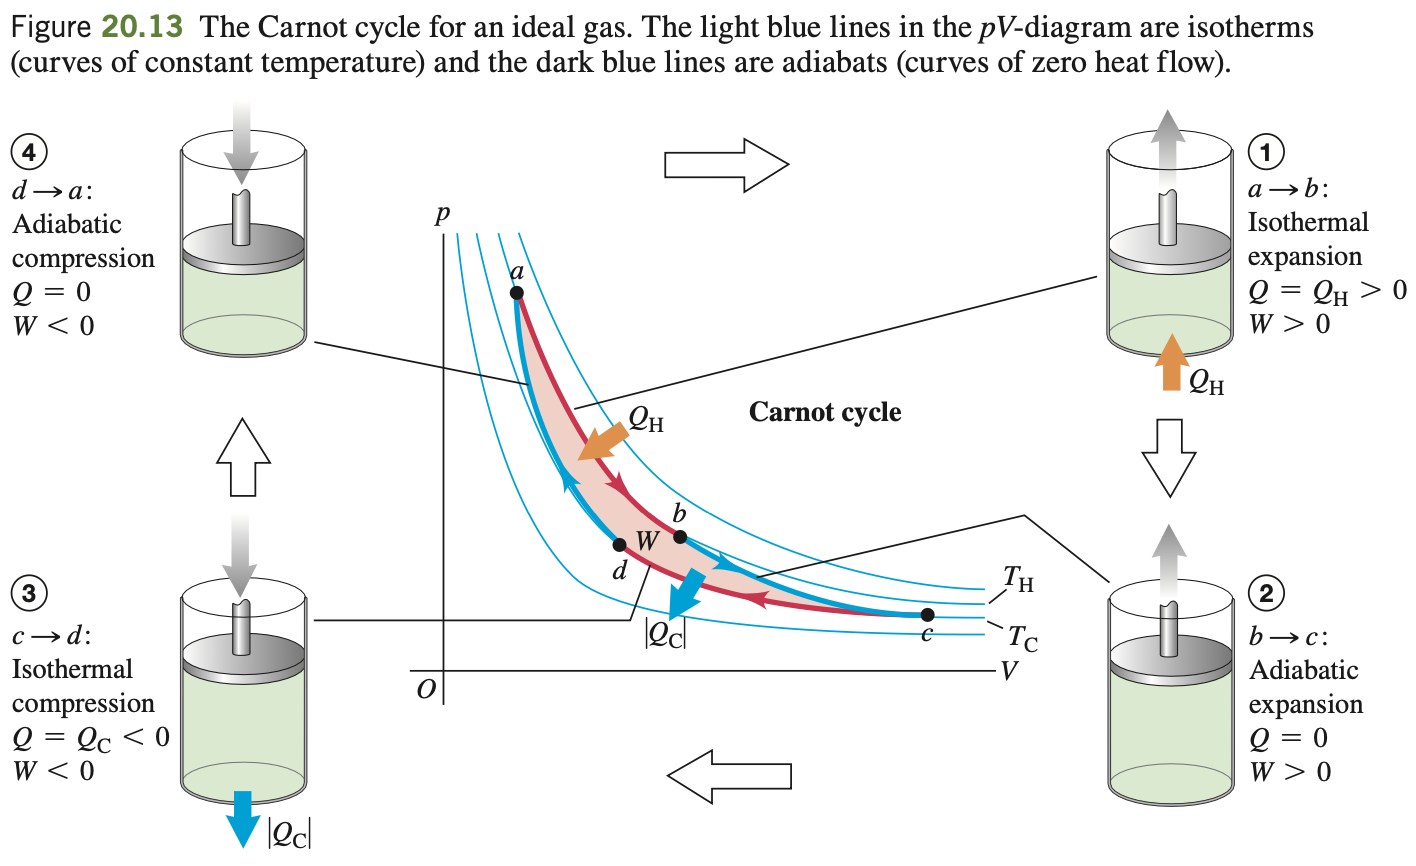
\includegraphics[scale=0.464]{carnot-cycle}

\begin{itemize}
  \item The amount of heat transferred to/from the reservoirs in a Carnot cycle are related to the temperatures of the reservoirs by \[\frac{Q_C}{Q_H} = -\frac{T_C}{T_H}.\]

  \item The efficiency of a Carnot engine is \[e_\text{Carnot} = 1 - \frac{T_C}{T_H}.\]

  \item Because all processes in the Carnot cycle are reversible, the cycle itself can be reversed to make a Carnot fridge.

  \item The coefficient of performance of a Carnot fridge is \[K_\text{Carnot} = \frac{T_C}{T_H - T_C}.\]
\end{itemize}

\subsection{Entropy}

\begin{itemize}
  \item \textbf{Entropy} $S$ is a measure of the randomness in a system. When you add heat to a system the constituent particles gain kinetic energy, there is more randomness to their positions, and thus entropy increases. When you remove heat from a system entropy decreases.

  \item The units of entropy are $\unit{J/K}$.

  \item The change in entropy during a reversible isothermal process is \[\Delta S = \frac{Q}{T}.\]

  \item The change in entropy during any reversible thermodynamic process can be calculated as \[\Delta S = \int_1^2 \frac{d Q}{T}\] where $\Delta S$ is the change in entropy, $1$ is the initial state, $2$ is the final state, $d Q$ is the infinitesimal heat flow into the system, and $T$ is the absolute temperature of the system.

  \item Entropy is determined entirely by the state of a system, not how it got there, i.e. entropy is path independent.

  \item In an adiabatic process $Q = 0$ and thus there is no change in entropy.

  \item To calculate the change in entropy of an irreversible process, come up with a series of reversible processes that take the system between the same states and calculate the change in entropy of that.

  \item When a system undergoes a reversible change from state $a$ to state $b$, the change in entropy is $0$. This means that the change in entropy of adiabatic and isothermal processes are $0$ (because they are reversible). The Carnot cycle is composed of adiabatic and isothermal processes so its change in entropy is also $0$. In general, the change in entropy for any reversible cyclic process is $0$.

  \item An alternative formulation of the second law of thermodynamics is that no process is possible in which total entropy decreases, when all systems that take part in the process are included.
\end{itemize}

\subsection{Microscopic Interpretation of Entropy}

\begin{itemize}
  \item A description of the \textbf{macroscopic state} of a system describes the system as a whole rather than individual components of the system, e.g. ``50\% of the coins are heads, 50\% are tails.''

  \item A description of the \textbf{microscopic state} of a system describes the individual components, e.g. ``Coin 1 is heads, coin 2 is tails, etc.''

  \item Many microscopic states may correspond to a given macroscopic state.

  \item For any thermodynamic system, the most probable macroscopic state is the one with the greatest number of corresponding microscopic states, which is also the macroscopic state with the greatest randomness and the greatest entropy.

  \item The entropy of a given macroscopic state is \[S = k \ln w\] where $k$ is the Boltzmann constant and $w$ is the number of microscopic states associated with the macroscopic state.
\end{itemize}

\setcounter{section}{36}
\section{Relativity}

\subsection{Invariance of Physical Laws}

\begin{itemize}
  \item \textbf{Einstein's first postulate} or the \textbf{principle of relativity} states that the law of physics are the same in every inertial frame of reference.

  \item \textbf{Einstein's second postulate} states that the speed of light in vacuum is the same in all intertial frames of reference and is independent of the motion of the source.

  \item It is not possible to travel at the speed of light.

  \item A \textbf{Galilean transformation} transforms between the coordinates of two reference frames that differ only by constant relative motion, e.g. \begin{align*}
          x & = x' + v t \\
          y & = y'       \\
          z & = z'.
        \end{align*}
\end{itemize}

\subsection{Relativity of Simultaneity}

\begin{itemize}
  \item In a given frame of reference an \textbf{event} is an occurence that has a definite position and time.

  \item In general, two events that are \textbf{simultaneous} in one frame of reference are not simultaneous in another frame that is moving relative to the first, even if both are inertial frames.
\end{itemize}

\subsection{Relativity of Time Intervals}

\begin{itemize}
  \item There is only one reference frame in which a given point is at rest and we call it the point's \textbf{rest frame}.

  \item The time interval measured between two events that occur at the same point (and thus in the point's reference frame) is called \textbf{proper time $\Delta t_0$}.

  \item The time interval between those two same events in another frame of reference moving at speed $u$ relative to the rest frame is \[\Delta t = \frac{\Delta t_0}{\sqrt{1 - u^2 / c^2}}\] which is greater than $\Delta t_0$. This phenomenon is called \textbf{time dilation}.

  \item The \textbf{Lorentz factor} is defined as \[\gamma = \frac{1}{\sqrt{1 - u^2 / c^2}}.\]

  \item If the relative speed $u$ of a reference frame is large enough that the Lorentz factor $\gamma$ is appreciably greater than $1$, the speed is said to be \textbf{relativistic}. Otherwise it's said to be \textbf{nonrelativistic}.
\end{itemize}

\subsection{Relativity of Length}

\begin{itemize}
  \item The length of a body as measured in its rest frame is called its \textbf{proper length $l_0$}.

  \item In a moving reference frame, The length of a body in the direction parellel to motion is \[l = \frac{l_0}{\gamma}\] which is less than $l_0$. This phenomenon is called \textbf{length contraction}.

  \item Length contraction doesn't occur in directions perpendicular to motion.
\end{itemize}

\subsection{The Lorentz Transformations}

\begin{itemize}
  \item If $S'$ is a reference frame moving at speed $u$ along the $x$-axis relative to reference frame $S$, then the \textbf{Lorentz transformation} can be used to determine the spacetime coordinates $x'$, $y'$, $z'$, and $t'$ in $S'$ from coordinates $x$, $y$, $z$, and $t$ in $S$ \begin{align*}
          x' & = \frac{x - u t}{\sqrt{1 - u^2 / c^2}} = \gamma (x - u t)              \\
          y' & = y                                                                    \\
          z' & = z                                                                    \\
          t' & = \frac{t - u x / c^2}{\sqrt{1 - u^2 / c^2}} = \gamma (t - u x / c^2).
        \end{align*}

  \item At relativistic speeds length and time have no meaning independent of a reference frame, so we use \textbf{spacetime coordinates} $x$, $y$, $z$, and $t$.

  \item The \textbf{Lorentz velocity transformation} can be used to determine the velocity in $S'$ in terms of the velocity in $S$ \[v_x' = \frac{v_x - u}{1 - u v_x / c^2}.\]
\end{itemize}

\subsection{The Doppler Effect For Electromagnetic Waves}

\begin{itemize}
  \item When the source of an electromagnetic wave of proper frequency $f_0$ is approaching a stationary observer at speed $u$, the observer measures frequency \[f = \sqrt{\frac{c + u}{c - u}} f_0.\] When the source is moving away from the observer the sign of $u$ changes.
\end{itemize}

\subsection{Relativistic Momentum}

\begin{itemize}
  \item The mass of a particle when it is at rest relative to the observer is called its \textbf{rest mass}.

  \item A particle's \textbf{relativistic momentum} is \[\mathbf{p} = \frac{m \mathbf{v}}{\sqrt{1 - v^2 / c^2}} = \gamma m \mathbf{v}.\] This means that as a particle's speed increases so does its relativistic momentum.

  \item The expression $\gamma m$ is sometimes called the \textbf{relativistic mass}, which increases with a particle's speed.

  \item Newton's second law must be adjusted at relativistic speeds. For forces parallel to the direction of motion \[F = \gamma^3 m a\] and for forces perpendicular to the direction of motion \[F = \gamma m a.\] This means that, unless the net force on a particle moving at relativistic speeds is either parallel or perpendicular to its direction of motion, the acceleration and force vectors aren't parallel.
\end{itemize}

\subsection{Relativistic Work and Energy}

\begin{itemize}
  \item The kinetic energy of a particle travelling at relativistic speeds is \[K = (\gamma - 1) m c^2.\]

  \item The total energy of a particle is \[E = \gamma m c^2\] or \[E^2 = (m c^2)^2 + (p c)^2.\]

  \item For a particle at rest $E = m c^2$. This is called the particle's \textbf{rest energy}.
\end{itemize}

\section{Photons: Light Waves Behaving as Particles}

\subsection{Light Absorbed as Photons: The Photoelectric Effect}

\begin{itemize}
  \item To escape from the surface of a material, an electron must absorb enough energy to overcome the attraction of positive ions in the material. The \textbf{photoelectric effect} is the phenomenon where light gives the electroncs this energy, producing a current.

  \item The maximum kinetic energy of an electron emitted via the photoelectric effect is \[K = \frac{1}{2} m v_\text{max}^2 = e V_0\] where $V_0$ is the \textbf{stopping potential}, i.e. the potential diffreence between the anode and cathode at which electrons no longer flow.

  \item The energy of a photon is \[E = h f = \frac{h c}{\lambda}\] where $h$ is \textbf{Planck's constant} \[h = \qty{6.62606957e-34}{J.s}.\]

  \item The maximum kinetic energy of an electron emitted via the photoelectric effect is \[e V_0 = h f - \phi\] where $\phi$ is the material's \textbf{work function}, i.e. the amount of energy required for an electron to overcome the attractive foces of ions.

  \item The momentum of a photon is \[p = \frac{E}{c} = \frac{h f}{c} = \frac{h}{\lambda}.\]
\end{itemize}

\subsection{Light Emitted as Photons: X-Ray Production}

\begin{itemize}
  \item Accelerated charges produce electromagnetic waves. When an electron is ``braked'' by a material it is decelerated, producing an electromagnetic wave. The frequency of that wave is determined by the charge's kinetic energy. If the charge is accelerated across a potential difference of $V$ then \[K = e V = h f = \frac{h c}{\lambda}.\]
\end{itemize}

\subsection{Light Scattered as Photons: Compton Scattering\\and Pair Production}

\begin{itemize}
  \item When a photon strikes an electron it gives up some of its energy and momentum to the electron and is redirected at an angle $\phi$ from its original path. The change in wavelength of the photon is given by \[\lambda' - \lambda = \frac{h}{m c} (1 - \cos \phi)\] where $\lambda'$ is the wavelength of the scattered photon, $\lambda$ is the original wavelength of the photon, $h$ is Planck's constant, $m$ is the mass of the electron, $c$ is the speed of light in vacuum, and $\phi$ is the scattering angle.

  \item If a gamma ray photon is fired at a target, it may not scatter. Instead it may disappear and be replaced with an electron / positron pair. A \textbf{positron} is a particle with the same mass as an electron but with opposite charge ($+e$).
\end{itemize}

\subsection{Wave-Particle Duality, Probability, and Uncertainty}

\begin{itemize}
  \item The \textbf{Heisenberg uncertainty principle} states that it is impossible to simultaneously determine both the position and momentum of a particle with arbitrarily great precision \[\Delta x \Delta p_x \ge \hbar / 2\] where $\Delta x$ is uncertainty in the $x$ coordinate, $\Delta p_x$ is uncertainty in the $x$ momentum, and $\hbar$ is Planck's constant divided by $2 \pi$.

  \item The Heisenberg uncertainty principle for energy and time is \[\Delta t \Delta E \ge \hbar / 2.\]
\end{itemize}

\end{document}